\chapter{PSD的宇宙线地面标定}
\label{ch:cosmic_ray}
PSD整体装配完成后,我们在实验室对它的各项性能指标进行了测试。
特别地,我们利用宇宙线对PSD所有的探测单元模块进行了细致的标定测试,得到了一系列的刻度参数结果。
这些结果是PSD得到的第一批刻度参数数据集,它们是PSD进行初步能量重建的基础。

我们专门研制并搭建了一套宇宙线地面标定测试平台,用于PSD的宇宙线标定测试。
本章将简单介绍该平台的基本组成以及它在PSD宇宙线标定中的应用,同时给出了PSD地面宇宙线标定的主要结果。

\section{宇宙线地面标定测试平台}
\label{sec:cosmic_ray:cm_system}
\subsection{简介}
\label{sec:cosmic_ray:introduction}
% 结构与组成,总装图
% 基本原理
宇宙线地面标定测试平台是专门为了PSD的地面标定而设计和建造的,主要提供了两个功能:1)模拟轨道真空环境;2)确定入射宇宙线径迹。
该平台的基本结构如图\ref{fig:cosmic_ray:cm_system}所示,其主体为一个大型真空靶室,
靶室的上部和下部分别放置了一个多丝漂移室探测器(Multi-Wire Drift Chamber,简称MWDC)和一个塑料闪烁体触发板探测器。
上下两块触发板用于标定入射宇宙线事例,而上下两个MWDC则用于测量入射宇宙线径迹。
根据得到宇宙线入射径迹,可以推出其在PSD上的击中位置。
由于MWDC和触发板的面积都能够覆盖PSD的有效探测面积,因此我们能够得到PSD所有位置处的MIP响应,从而实现PSD的精细标定。
\begin{figure}[htbp]
	\centering
	\includegraphics[width=0.9\textwidth]{chap/cosmic_ray/fig/cm_system_schematic.png}
	\caption{宇宙线地面标定系统的硬件组成}
	\label{fig:cosmic_ray:cm_system}
\end{figure}

按照功能分类,该测试平台可以被分为真空系统、径迹探测系统、触发系统以及数据获取系统四个功能模块。
下面,依次对各个分系统进行详细介绍。

\subsection{真空系统}
\label{sec:cosmic_ray:vacuum_system}
% 靶室大小,结构包括滑台,外观图
% 高压法兰,信号法兰图
% 真空泵,参数
真空系统主要由靶室、真空泵以及真空检测设备组成。
靶室腔体可以容纳整个PSD探测器;靶室外部支架上设计有托盘,用于固定MWDC和塑闪触发板。
靶室内部还铺设了两根导轨,操作时,我们先将PSD安放在一个铝合金滑台上并准确定位,然后将滑台沿着导轨推入到靶室腔体中,最后将滑台用卡扣卡住以防其滑动。这样不仅方便了PSD的放置操作,而且能够准确定位PSD在靶室内部的位置,为后面的数据分析提供依据。
为了给靶室内部的PSD提供高压并将其信号引出,我们专门加工了PSD专用的高压转接法兰和信号转接法兰。

真空系统中的真空泵设备由机械泵和分子泵两级组成,以保证靶室内部可以达到较高的真空度。
由于靶室体积较大,我们配备了两套相同的真空泵设备,以加快抽真空的速度。
实际使用中发现:当靶室内部放置了PSD探测器和相应的连接线缆后,上述设备可以在24小时内将靶室内部真空抽取到\SI{0.01}{Pa}的量级。

\subsection{径迹探测系统}
\label{sec:cosmic_ray:tracking_system}
% MWDC工作原理
径迹探测系统由两个完全一样的大面积多丝漂移室(MWDC)探测器组成。
MWDC是气体探测器的一种,由于制造成本低廉、操作简单以及位置分辨较高,它是粒子物理实验中最常用的位置灵敏探测器之一。
MWDC一般由多个漂移单元组成,每个漂移单元都是MWDC进行位置测量的最小单位。
一个漂移单元由位于中心的一根阳极丝和周围的若干根阴极丝组成;工作时,阳极丝加正高压(或接地),而阴极丝接地(或加负高压);阴极丝也被称为场丝,因为它们的排布方式决定了漂移单眼内部的电场分布。
入射粒子穿过漂移单元时,在其中发生的物理过程可以叙述如下:
\begin{enumerate}
	\item 入射粒子使得单元内的气体分子电离,从而产生自由的电子离子对。
	\item 在电场作用下,电离出来的电子被加速并缓慢向阳极丝漂移,而离子则向阴极丝移动。
	\item 由于阳极丝附近电场强度非常大,自由电子漂移到这个区域以后迅速被加速到足够高的能量并能够引发新的电离。这个过程不断地反复地进行,从而产生大量电离电子,这个现象被称为雪崩效应。
	\item 雪崩效应产生的自由电子继续向阳极丝移动,由于距离阳极丝非常近,它们立即被阳极丝收集。
	\item 与此同时,原初电离以及次级电离产生的正离子继续向阴极丝移动,由于离子的质量大,它们的漂移速度很慢,而且也不会在阴极丝附近产生雪崩效应。
\end{enumerate}
上述各个步骤中,只有大量雪崩电子向阳极丝移动并被迅速吸收这个过程能够使得阳极丝上的电荷分布发生变化并感应出幅度可探测的电流脉冲信号。
MWDC探测到的也就是这个阳极丝上的感应电流信号,该信号产生时刻与入射粒子穿过漂移单元的时刻的时间差就是原初电离电子的漂移时间。
由于漂移距离与漂移时间直接关联,通过测量漂移时间可以反推出原初电离位置相对于阳极丝的位置,这就是MWDC进行位置测量的基本原理。

% 基本结构:面积,丝参数,精度。
% MWDC结构示意图(丝距离,丝面排布)
% MWDC实物图
宇宙线标定测试平台中使用的MWDC探测器由X,Y,U三个方向的漂移单元平面阵列组成,其有效探测面积为$840mm \times 840mm$。
X面与Y面成\SI{90}{\degree}排布,它们内部都有80个漂移单元;U面与X面成\SI{30}{\degree}排布,它的内部有106个漂移单元,如图\ref{fig:cosmic_ray:mwdc_schematic}中的(a)所示。
漂移单元平面阵列是由两个阴极面和一个阳极面构成的,面间距为\SI{5}{mm}。
其中,阴极面由直径为\SI{100}{\micro\meter}的铍铜丝紧密排列组成,而阳极面由直径为\SI{100}{\micro\meter}的铍铜丝和直径为\SI{20}{\micro\meter}的镀金钨丝间隔排列组成,如图\ref{fig:cosmic_ray:mwdc_schematic}中的(b)所示。
\begin{figure}[htb]
\centering
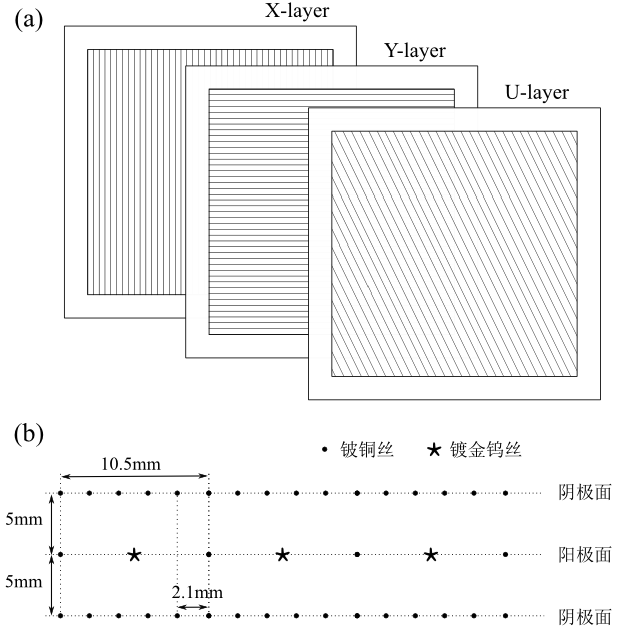
\includegraphics[width=0.65\textwidth]{chap/cosmic_ray/fig/mwdc_schematic.png}
\caption{MWDC内部结构:a)X,Y,U三个方向的漂移单元阵列;b)漂移单元阵列内的丝面排布方式}
\label{fig:cosmic_ray:mwdc_schematic}
\end{figure}
工作时,所有的铍铜丝加负高压,它们是漂移单元的阴极丝;所有的镀金钨丝接地,它们是漂移单元的阳极丝。
因此,根据图\ref{}给出的间距,可以得到MWDC的漂移单元是一个截面为$10mm\times 10.5mm$的长方体。
MWDC探测器的工作气体为$\SI{20}{\percent}CO_2 + \SI{80}{\percent}Ar$,整个漂移腔体用Kapton膜密封,图\ref{fig:cosmic_ray:mwdc}给出了一个MWDC探测器的实物图。
\begin{figure}[htbp]
	\centering
	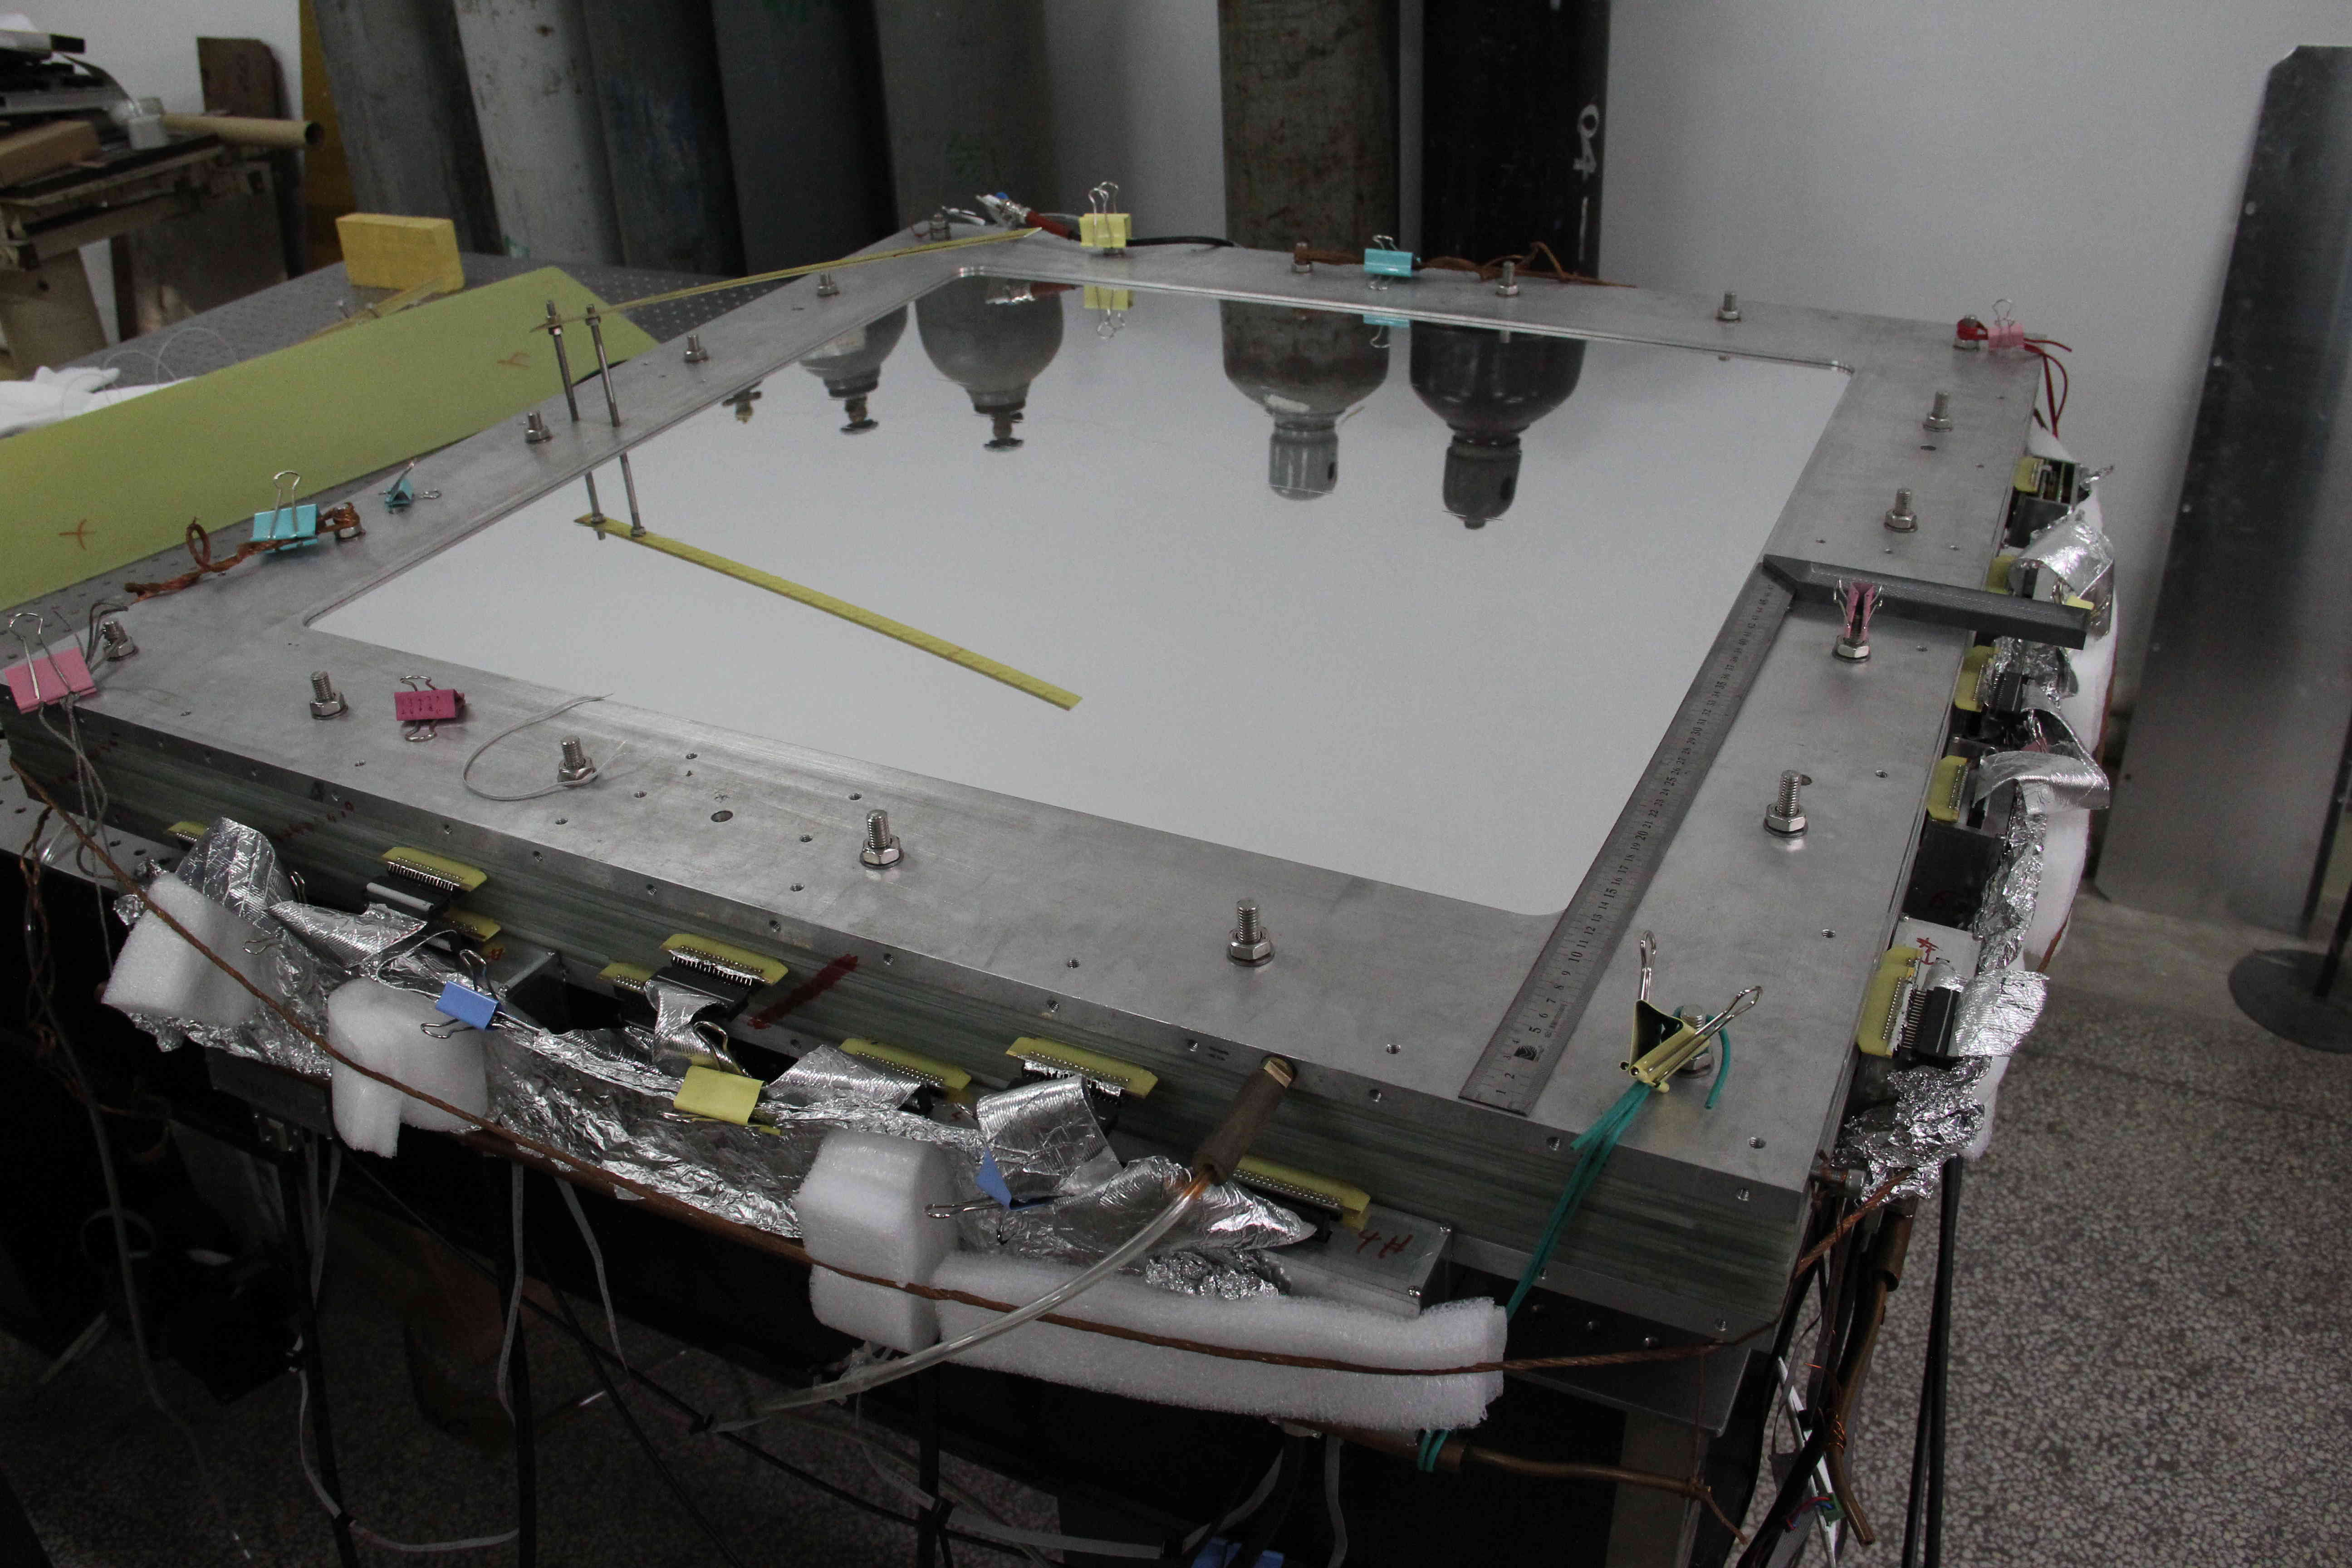
\includegraphics[width=0.65\textwidth]{chap/cosmic_ray/fig/mwdc.jpg}
	\caption{MWDC实物图}
	\label{fig:cosmic_ray:mwdc}
\end{figure}

% MWDC的信号处理系统
MWDC的输出信号幅度较小,为了提高信噪比,我们使用一块基于SFE16芯片的前端电子学板对原始信号进行预处理,然后才将其输出到数据获取系统中进行时间测量(见\ref{sec:cosmic_ray:daq_system}节)。
SFE16是一款专门用于气体漂移室前端信号处理的低噪声ASIC芯片。
它将16个测量通道集成在一块芯片上,每个通道都具有信号放大和甄别的功能,因此输出信号可以直接用于时间测量,并适合长距离传输。
关于SFE16的详细信息可以参考文献\parencite{sfe16}。

\subsection{触发系统}
\label{sec:cosmic_ray:triggering_system}
% 触发板结构,面积,厚度,四角读出,实物图?
触发系统由两块完全一样的塑料闪烁体触发板探测器组成。
触发板探测器使用\SI{30}{mm}厚的塑料闪烁体EJ-200\parencite{ej-200}作为探测介质,探测器形状为正方形,有效面积为$825mm \times 825mm$。
塑闪板表面抛光,并在内层包裹Tyvek纸以提高反射效率,而在外层包裹黑胶带以屏蔽外界的光干扰。
最后,塑闪板的四个角各耦合了一支光电倍增管,用于闪烁光信号读出。
使用的光电倍增管型号为Hamamatsu公司的R7724\parencite{r7724}。

% 触发板的信号处理系统
触发系统具有两个功能:1)标识入射宇宙线,为数据获取系统提供触发信号;2)用于宇宙线击中时刻的测量,为MWDC漂移时间的计算提供时间零点。
上下两块触发板探测器共有8路信号输出,相应地,它们经过甄别后可以得到8路时间信号。
每一路时间信号都扇出两路,一路信号参加8路时间信号的逻辑与运算;另一路信号用于时间测量。
上述两个功能都在同一块信号处理板中实现,详细内容参看\ref{sec:cosmic_ray:daq_system}节。
我们认为真实的宇宙线事例应该使得上下两块触发板都点火,因此8路信号相与得到的输出信号将作为触发信号输入到数据获取系统中以记录该事件。
而8个角上得到的时间测量值将被用于漂移时间零点的计算。

% 响应均匀性,击中位置图或者唐述文文章中的图
由于触发板的面积较大,宇宙线击中板上不同位置处产生的闪烁光传输到塑闪板角上PMT的时间是有差异的,我们把这个现象称为时间测量不均匀性,如图\ref{fig:cosmic_ray:tof_timeVSposition}所示。
\begin{figure}[htbp]
	\centering
	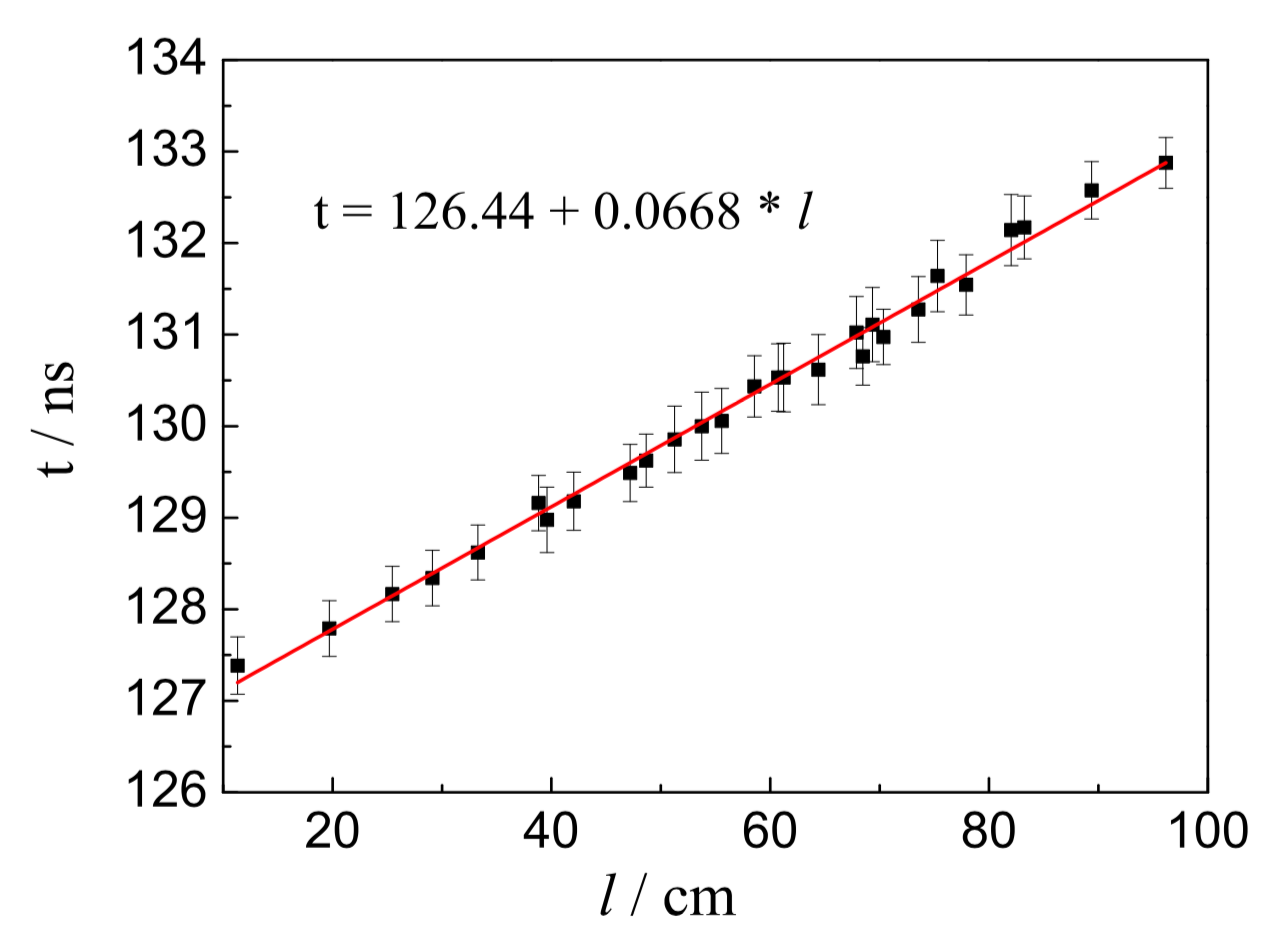
\includegraphics[width=0.65\textwidth]{chap/cosmic_ray/fig/tof_timeVSposition.png}
	\caption{触发板的时间测量不均匀性,引自\parencite{tang_large_2015}。其中,纵轴是某个角得到的击中时刻,而横轴是击中位置距离这个角的直线距离。拟合直线斜率的倒数就是闪烁光在塑闪板中的有效传播速度。}
	\label{fig:cosmic_ray:tof_timeVSposition}
\end{figure}
这意味着,我们不能简单地选择一支PMT的时间信号作为时间零点,因为这会带来较大的时间晃动,影响漂移时间的测量精度。
为了消除时间测量不均匀性,必须综合板上四个角的时间测量信息,以使得时间零点与击中位置无关。
实际中,我们使用下列形式\parencite{annand_large_1987}得到时间零点$T_{eff}$:
\begin{equation}
	T_{eff} = \frac{1}{4}\sum^4_{i=1}T_i - \frac{v_{eff}}{8d}[(T_3-T_1)^2+(T_4-T_2)^2]
	\label{eq:cosmic_ray:tof_time}
\end{equation}
其中,$v_{eff}$是闪烁光在塑闪板中有效传输速度,$d$是塑闪板的对角线长度,$T_1\sim T_4$是塑闪板四个角的时间测量值,并且$T_1$和$T_3$是对角,而$T_2$和$T_4$也是对角。
测试发现,使用公式\ref{eq:cosmic_ray:tof_time}得到的塑闪板时间分辨率可以达到\SI{350}{\pico\second}\parencite{tang_large_2015}。

\subsection{数据获取系统}
\label{sec:cosmic_ray:daq_system}
% PXI机箱图,触发板,MWDC板,TOF板
数据获取系统基于PXI总线设计,主要由触发板,时钟板,TOF测量板以及MWDC测量板组成\parencite{kanglongfei_thesis,zhoujiawen_thesis}。
这些板卡都安装在一个6U高,具有15个槽位的PXI机箱中\parencite{pxi_chassis},而获取和控制软件安装在机箱第一个槽位的单片机上。
下面,对这四种板卡的功能进行简单的介绍。

TOF测量板和MWDC测量板是数获取系统进行时间测量的核心模块,其中TOF板用于触发板探测器的时间测量,而MWDC板用于MWDC探测器的时间测量。
两块测量板都是基于HPTDC芯片设计的,能够在高计数率条件下对时间进行精确测量。
HPTDC是欧洲核子中心(CERN)开发的一款高性能时间测量ASIC芯片\parencite{hptdc_manual}。
与以往核物理实验中常见的起停式时间测量方法不同,HPTDC直接测量输入时间信号的到达时刻,而不是测量输入时间信号与触发信号的时间差。
HPTDC也需要触发信号,但它并不将触发信号作为时间测量的零点,而是使用触发信号来寻找真实的时间测量值,具体流程如下:
\begin{enumerate}
	\item 首先,任何输入到HPTDC的时间信号,不管是真实物理事件产生的还是本底噪声产生的,它们的到达时刻都会被测量并暂时保存到芯片的信号缓存区中。
	\item 之后,触发信号输入到HPTDC中,其到达时刻也被测量并暂时保存到触发信号缓存区中。
	\item 由于触发信号代表真实的物理事件,它的产生时刻与真实待测的时间信号之间必定满足一定的时间关系(包括各种电子学和线缆的延迟时间)。这个关系可以用一个时间窗口来表示,并可以在实验前通过模拟和测试估算出来。用户在实验开始前,需要将这个关系配置保存到在HPTDC的配置寄存器中。
	\item 实验中,HPTDC就是根据这个配置好的时间窗口,从信号缓存区中已有的时间测量值中找到每个触信号对应的真实时间测量值,并将其输出到读取FIFO中,供获取软件使用。
\end{enumerate}
由于HPTDC会将信号缓存区中所有在时间窗口内的测量值都提取出来,因此需要仔细调节时间窗口配置以达到每个触发信号只能找到一个测量值的最佳状态。
这给实验准备提出了更高的要求,但这种测量方法具有死时间小、配置灵活等优点,非常适合复杂探测器系统在高计数率条件下的使用。
HPTDC具有32个测量通道,每个通道的时间测量精度为\SI{98}{\pico\second};HPTDC也可以工作在精度为\SI{25}{\pico\second}的甚高精度模式下,此时每4个测量通道合并成1个测量通道,即此时HPTDC只有8个测量通道。
TOF板共有16个测量通道,其内部共使用了3片HPTDC,其中两片用于时间测量,工作在甚高精度模式下,一片用于TOT幅度测量(Time-Over-Threshold),工作在正常模式下。
MWDC板共有128个测量通道,其内部使用了4片HPTDC,全部工作在正常模式下。

TOF测量板在时间测量模块之前还加入了甄别模块。
这样,来自PMT的原始信号可以直接输入到TOF板中,它们首先经过甄别模块的处理被转换成时间信号,然后才会输入到HPTDC芯片中。
而MWDC测量板不需要添加额外的甄别模块,因为MWDC探测器原始信号的甄别工作在前端电子板中就已经完成(见\ref{sec:cosmic_ray:tracking_system}节)。
另外,TOF测量板还能够依次对相邻两路输入通道的时间信号做逻辑与运算,然后将得到的8个与运算结果再作或运算,并将最终结果从前面板输出。

由于HPTDC只能测量时刻值,为了得到漂移时间,我们需要将MWDC板测得的信号时刻减去TOF板测得的宇宙线击中时刻。
这就要求不同测量板内的HPTDC芯片参考时钟是同步的,这样我们才能将不同测量板的时间测量结果直接相减。
时钟板的功能就是输出16路完全同步的\SI{40}{Hz}时钟信号。
这些时钟信号通过等长的时钟信号线缆输入到每块测量板中,这样所有测量板就有了统一的参考时钟信号,它们的测量结果也就能够直接进行对比了。

触发板主要有两个功能:1)接收外部触发信号,然后将该触发信号同步地分发到各块测量板中;2)将HPTDC的时间重置命令同步发送到各块测量板。
其中,时间重置命令的同步发送对不同测量板的时间测量同步性至关重要。
为了保证严格的同步性,触发板安装在PXI机箱的2号槽位中,并使用PXI机箱背板上的星形触发总线来进行触发信号
和时间重置信号的分发。
星形触发(Star Trigger)是PXI总线的主要特点之一,PXI机箱的第二个槽位是星形触发控制器槽,该槽位到达其它13个槽位的走线长度是等长的,因此可以实现信号分发严格同步。

% \section{多丝漂移室的宇宙线刻度}
% \subsection{漂移时间零点的确定}
% \subsection{从漂移时间谱提取s-t关系:Integration Method}
% \subsection{迭代修正s-t关系}
% \subsection{多丝漂移室的性能参数}

\section{PSD的宇宙线标定测试配置}

% 15天,23个/s,一共事例数? 27%左右的单根丝点火事例
我们使用上述宇宙线地面标定系统对PSD进行了长达半个月的宇宙线标定测试。
测试时,PSD被安置在真空靶室中,靶室内真空一直保持在\SI{e-2}{Pa}水平,PSD的各探测单元模块加载额定工作电压。
整个测试期间,PSD各功能模块工作稳定,也没有发现PSD发生高压打火的现象。

% 与PSD系统的集成,触发Veto板。
PSD和宇宙线标定测试平台的数据获取系统在硬件和软件上都是完全独立的,两者各自获取一份数据并保存在不同的计算机中,如图\ref{fig:cosmic_ray:cm_test}所示。
\label{sec:cosmic_ray:cm_test}
\begin{figure}[htbp]
	\centering
	\includegraphics[width=0.65\textwidth]{chap/cosmic_ray/fig/cm_test.jpg}
	\caption{PSD的宇宙线标定测试。图中真空靶室还未上盖,靶室左边是宇宙线标定测试平台的数据获取系统,靶室前部是PSD的地面检测获取系统。}
	\label{fig:cosmic_ray:cm_test}
\end{figure}
这就涉及到两个系统的同步问题:我们将同一个触发信号同时分发到两个获取系统中,并期望两者能够同时处理完这个事例,并一起等待下个触发信号的到来。
为此,我们开发了一块触发Veto板,它接收来自触发系统的宇宙线触发信号,然后将其扇出两路,并分别输出到PSD
和宇宙线标定测试平台的数据获取系统中。
与一般的触发分发不同的是,该触发Veto板在接收一个有效触发信号并分发出去后,它在一定的时间间隔内不再接收新的触发信号,即屏蔽这段时间内的所有宇宙线触发事例。
如果将这个屏蔽时间设置为两个获取系统的最大死时间,我们就可以保证两个系统在接收到下个触发信号前都完成了前一个事例的处理,从而强制实现了两者的同步。
这种同步方法是被动的,如果屏蔽时间设置的过大,就可能导致部分有效事例丢失。
实际中,我们将触发Veto板的屏蔽时间设置为\SI{1}{ms},即PSD获取系统的死时间。
由于宇宙线事例的触发率远小于\SI{1000}{\per\second},该屏蔽时间设置基本不会导致事例丢失。

% 触发板预支设置,击中分布图
测试前,我们还对触发系统的8个读出PMT的工作电压进行了调节和测,原则是:1)在不增加噪声的前提下,尽量升高PMT的工作电压,提高增益系数,达到提高触发效率的目的;2)调节同一块触发板4个角读出PMT的电压,使得它们的增益基本一致,达到不同击中位置的触发效率基本一致的目的。
最终,在实际测试中,触发系统的宇宙线触发效率达到了\SI{27}{\per\second},并实现了较好的触发效率均匀性。
图\ref{fig:cosmic_ray:hitposition}给出了靶室上方MWDC探测器的宇宙线击中位置分布图,靶室下方的MWDC探测器也有类似结果。
\begin{figure}[htb]
\centering
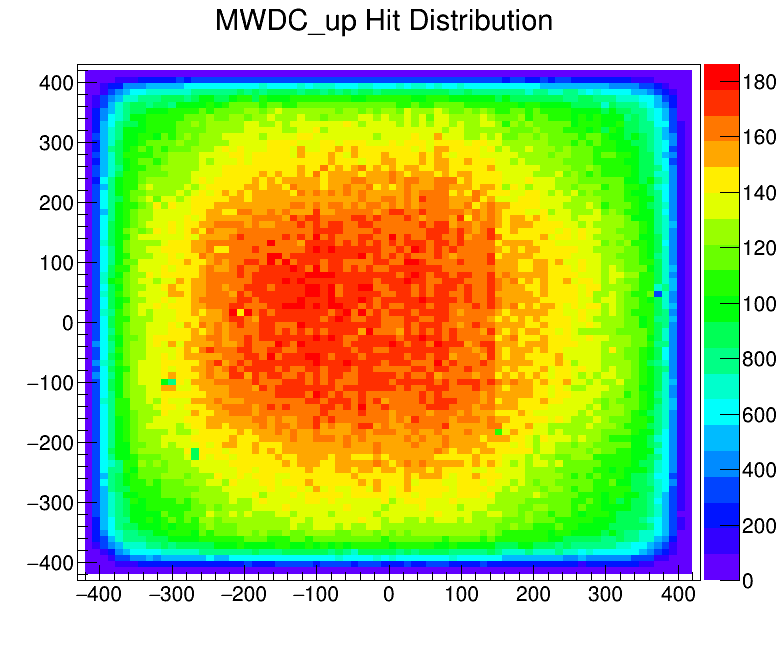
\includegraphics[width=0.6\textwidth]{chap/cosmic_ray/fig/hitposition_mwdc.png}
\caption{触发系统的触发效率均匀性}
\label{fig:cosmic_ray:hitposition}
\end{figure}
可以看到,击中位置分布呈现出中间多,边缘少的特点,这是因为两块触发板距离较远,中间位置的接收角度远大于边缘位置。
同时可以看到,击中位置在四周,尤其是4个角上的分布基本均匀,这说明不同位置处的触发效率基本是一致的。

\section{PSD的宇宙线标定结果}
\label{sec:cosmic_ray:results}
\subsection{基线噪声}
\label{sec:cosmic_ray:pedestal}
% 加高压与未加高压的结果对比。
% 基线中心值。
% 电子学刻度,噪声转换成电荷TODO
PSD加上额定工作电压后,我们首先对基线噪声进行了刻度,方法如下:使用信号发生器产生频率为\SI{100}{Hz}的周期性触发信号,并将其输入到PSD的地面检测数据获取系统中。
由于该触发信号与宇宙线击中PSD的事件间偶然符合的概率非常小,这样采集到的数据就是各个电子学通道的基线,而基线的展宽就代表对应电子学通道的噪声大小。
图\ref{fig:cosmic_ray:sigam_dist}给出了PSD所有328个探测器通道的基线噪声分布。
可以看到,PSD的噪声非常小,所有通道的噪声都小于5道。
\begin{figure}[htbp]
	\centering
	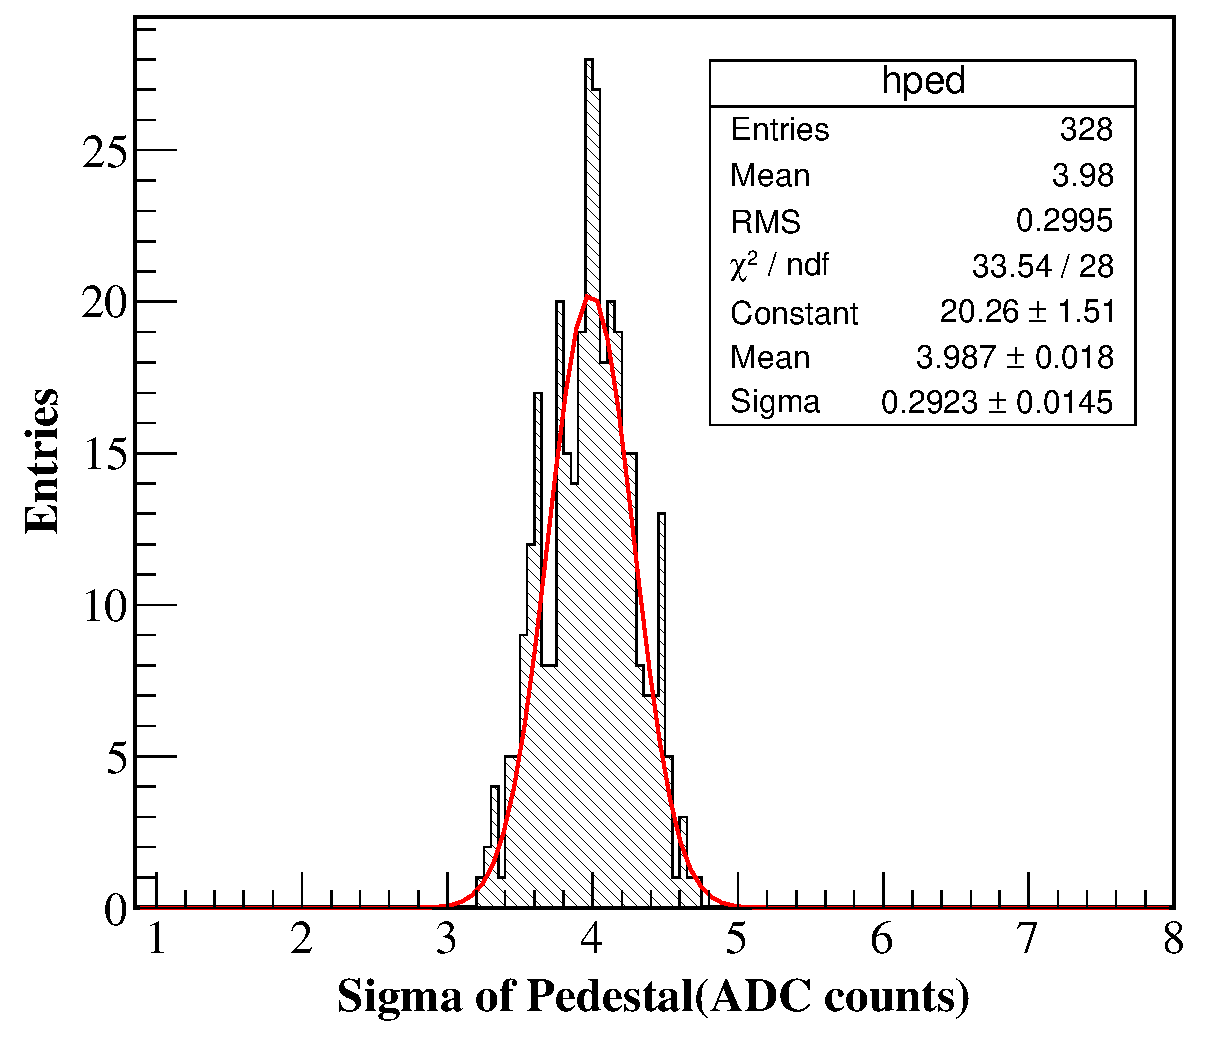
\includegraphics[width=0.55\textwidth]{chap/cosmic_ray/fig/sigam_dist.eps}
	\caption{PSD所有探测通道的基线噪声分布}
	\label{fig:cosmic_ray:sigam_dist}
\end{figure}

在PSD的宇宙线标定期间,我们每天都会进行两次的基线噪声刻度,结果显示PSD的基线噪声非常稳定,基本没有大的波动。
这表明真空环境并没有给PSD的工作带来影响,PSD的相关设计是合理的。

\subsection{MIP能量响应}
\label{sec:cosmic_ray:mip}
% 测量结果的修正叙述
对于PSD的每个探测单元模块,我们通过筛选出击中塑闪单元条中间位置\SI{20}{mm}区间的宇宙线事例,得到它们的中间位置MIP能量响应。
为了得到更加准确的结果,对于每个有效事例,我们还根据宇宙线径迹的入射角度大小对其沉积能量进行了修正。
这是因为,不同入射角度的宇宙线,它们所穿过的单元条厚度是不一样的。
由于宇宙线在PSD单元条内的沉积能量与其穿过的单元条厚度成正比,因此不同入射角度的宇宙线在PSD单元条内的沉积能量也是不一样的。

\begin{figure}[htbp]
	\centering
	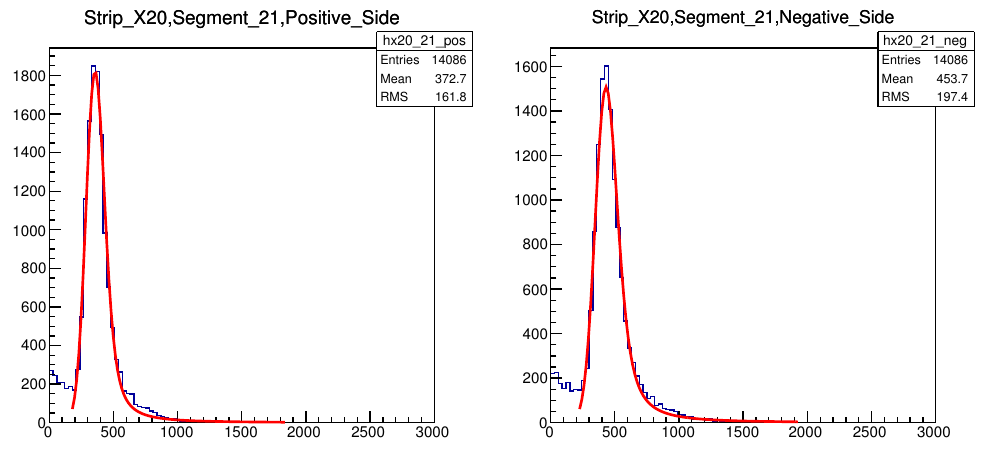
\includegraphics[width=0.95\textwidth]{chap/cosmic_ray/fig/mip_example.png}
	\caption{PSD第X层第21个探测单元模块中间位置的MIP能量响应原始谱,其中横轴是ADC道数,纵轴是事例数}
	\label{fig:cosmic_ray:mip_example}
\end{figure}
图\ref{fig:cosmic_ray:mip_example}给出了此次标定测试得到的一个结果示例,它是PSD第X层第21个探测单元模块两端得到的中间位置MIP能量响应原始谱。
使用朗道函数对谱线进行拟合(如图中红线所示),可以得到该探测单元模块的MIP能量响应的中心值(即朗道分布的MPV值)和能量分辨率(即朗道分布的Sigma值除以MPV值)。

使用上述方法,我们得到了PSD所有探测单元模块中间位置的MIP能量响应中心值和能量分辨率,它们的分布如图\ref{fig:cosmic_ray:mip_results}所示。
可以看到,PSD所有探测单元模块的MIP能量响应中心值集中分布在$[300,450]$道之间,一致性达到了\SI{10}{\percent};而PSD所有单元的能量分辨率都在\SI{10}{\percent}左右,远远好于PSD的设计要求\SI{25}{\percent}。
\begin{figure}[htb]
\centering
\subfloat[][能量响应一致性]{
	\label{fig:cosmic_ray:consist_dist}
	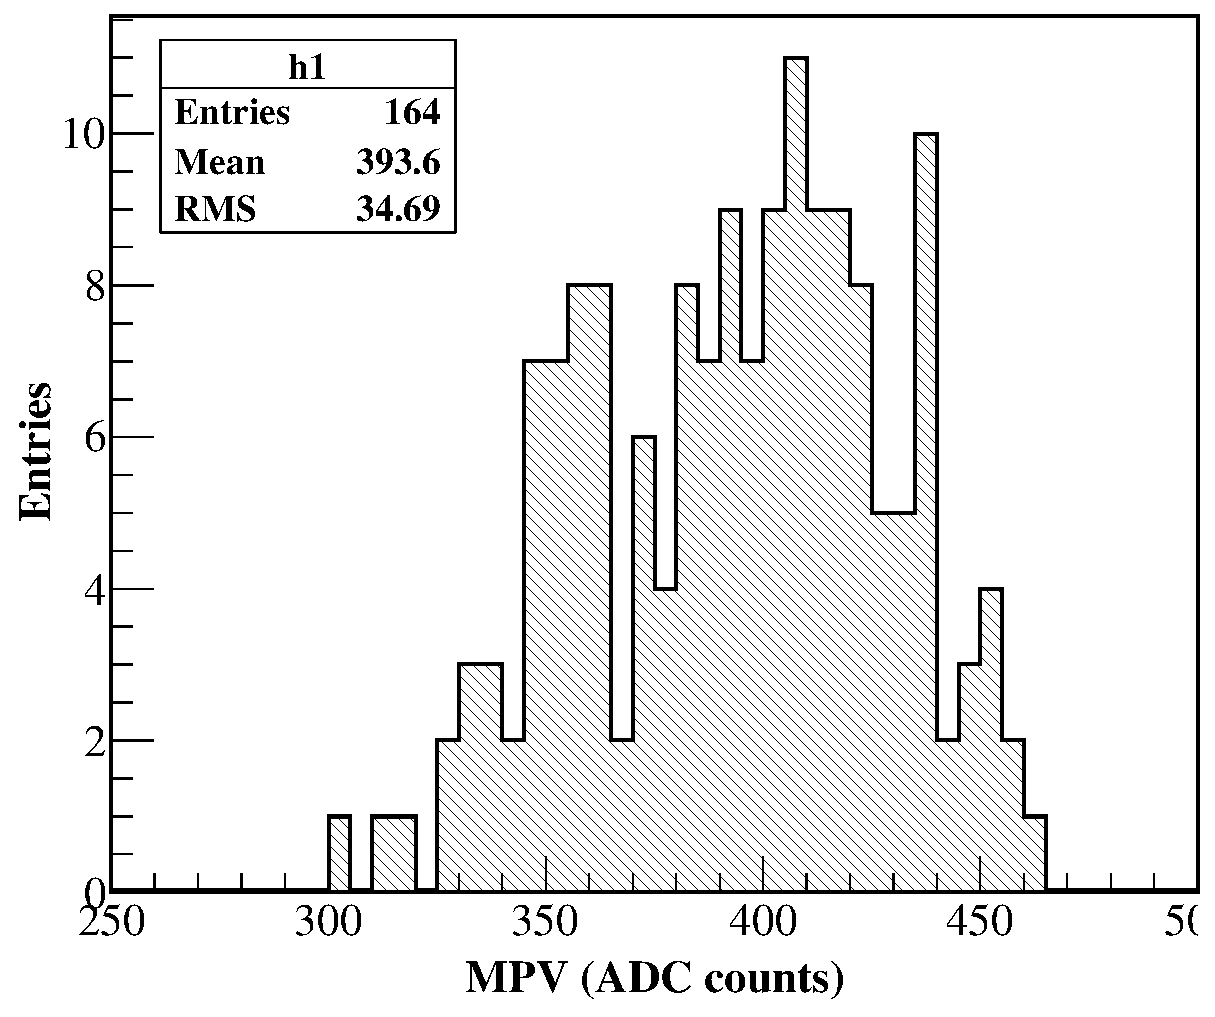
\includegraphics[width=0.48\textwidth]{chap/cosmic_ray/fig/consist_dist.eps}
}
\subfloat[][MIP能量分辨率]{
	\label{fig:cosmic_ray:energy_res_dist}
	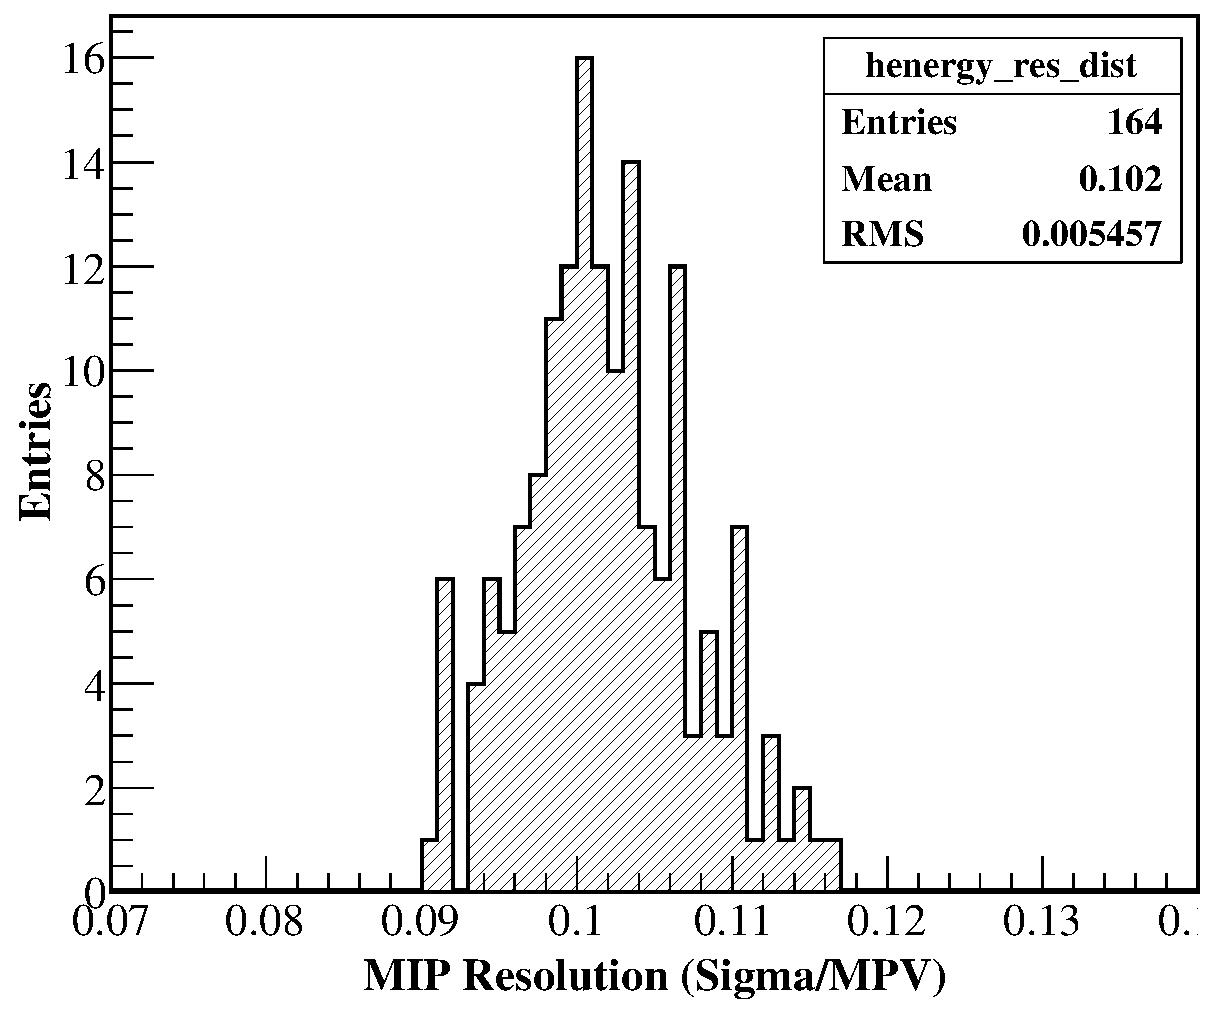
\includegraphics[width=0.48\textwidth]{chap/cosmic_ray/fig/energy_res_dist.eps}
}
\caption{PSD所有探测单元模块的MIP能量响应测试结果}
\label{fig:cosmic_ray:mip_results}
\end{figure}
% 中心MIP拟合示例图
% 中心值一致性
% 能量分辨率分布

\subsection{光衰减效应}
\label{sec:cosmic_ray:attenuation}
为了考察光衰减效应,我们将探测单元模块\SI{820}{mm}的有效探测长度分为41个位置区间,每个区间长度为\SI{20}{mm}。
在每个位置区间内,使用\ref{sec:cosmic_ray:mip}节的方法得到该位置的MIP能量响应中心值。
将这41个位置区间的能量响应中心值综合在一起,我们就得到了探测单元模块的光衰减曲线。
图\ref{fig:cosmic_ray:attenuation_example}是此次标定测试得到的一个结果示例。
\begin{figure}[htbp]
	\centering
	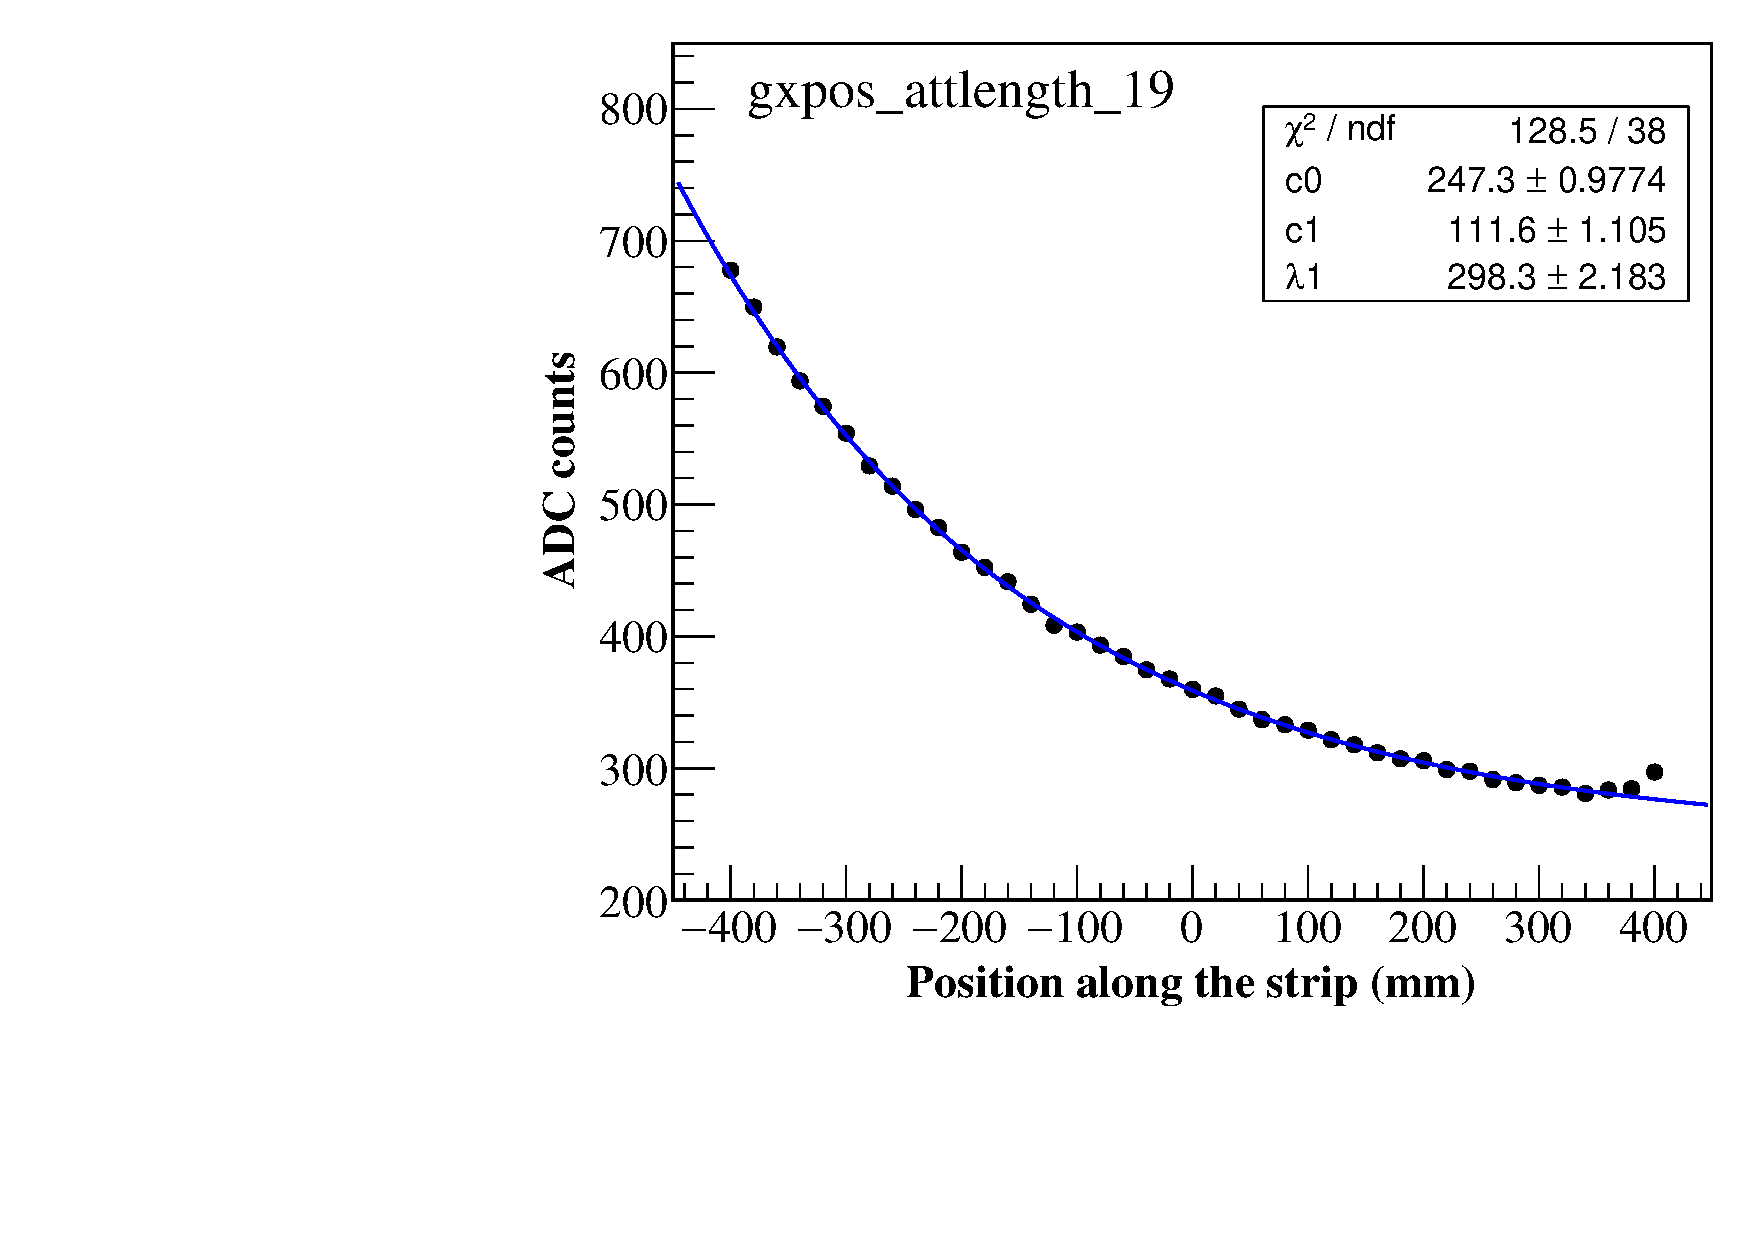
\includegraphics[width=0.60\textwidth]{chap/cosmic_ray/fig/attenuation_example.pdf}
	\caption{X层第19个探测单元模块正端得到的光衰减曲线,横轴是击中位置在单元条上的坐标,纵轴是对应位置的MIP能量响应中心值}
	\label{fig:cosmic_ray:attenuation_example}
\end{figure}
我们发现简单形式的指数衰减规律不能够解释PSD的光衰减曲线,尤其在单元条的端头位置。
因此,我们使用了公式\ref{eq:dynamic_range:attenuation}对上述数据点进行拟合,如图中蓝线所示,该公式可以很好地描述测试数据。

使用上述方法,我们得到了所有探测单元模块正负两端的光衰减曲线,并使用公式\ref{eq:dynamic_range:attenuation}拟合测试数据。
根据拟合结果,我们进一步计算了每个探测单元模块最远端和最近端相对于中间位置的光输出强度比值,结果如图\ref{fig:cosmic_ray:atten_dist}所示,
\begin{figure}[htb]
\centering
\subfloat[][最近端相对于中间位置的光输出强度比值分布]{
	\label{fig:cosmic_ray:atten_dist_max_mid}
	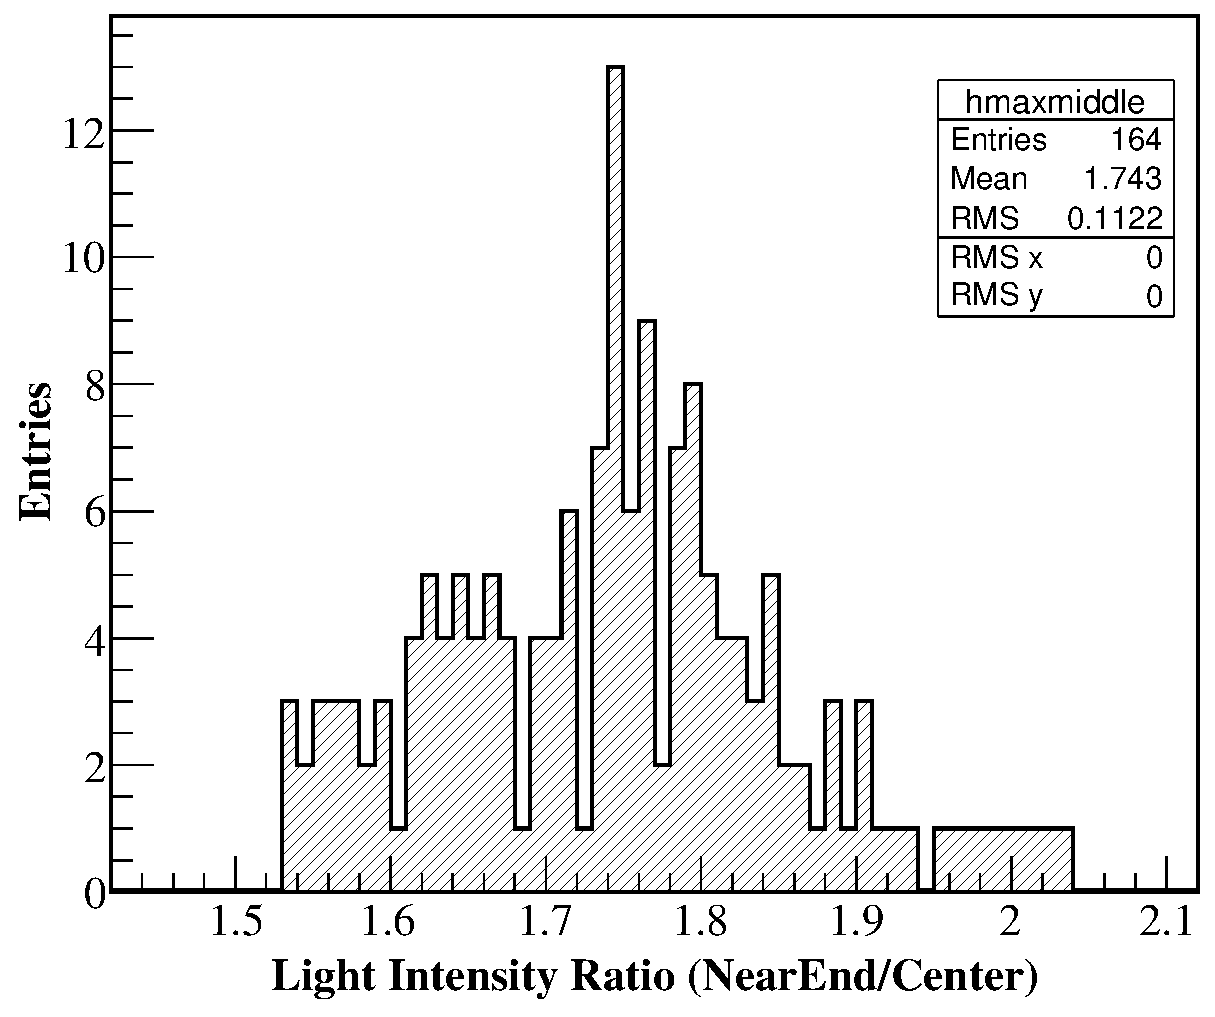
\includegraphics[width=0.48\textwidth]{chap/cosmic_ray/fig/atten_dist_max_mid.eps}
}
\subfloat[][中间位置相对于最远端的光输出强度比值分布]{
	\label{fig:cosmic_ray:atten_dist_mid_min}
	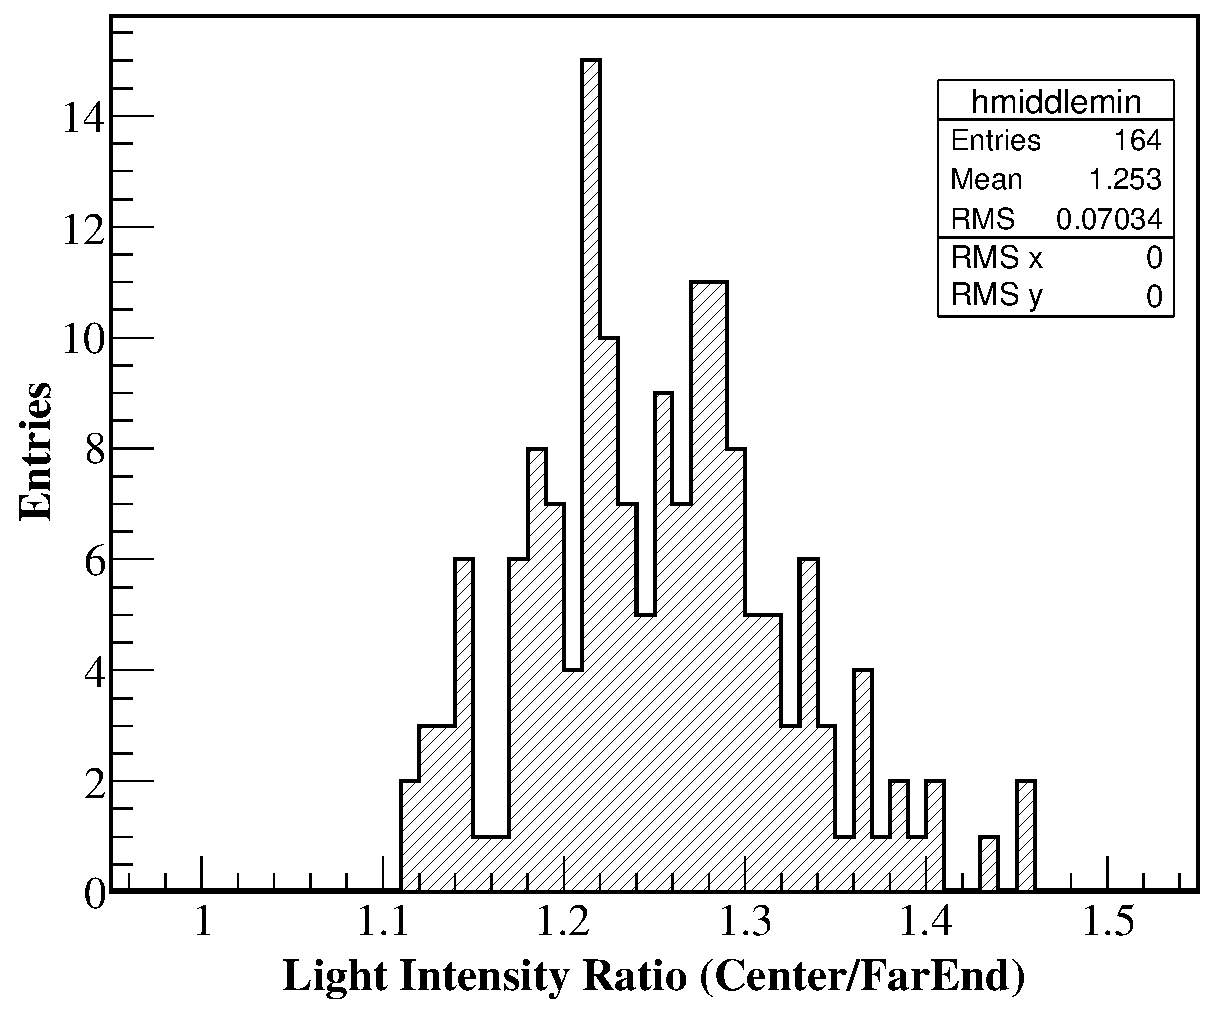
\includegraphics[width=0.48\textwidth]{chap/cosmic_ray/fig/atten_dist_mid_min.eps}
}
\caption{PSD所有单元模块的光衰减效应分布}
\label{fig:cosmic_ray:atten_dist}
\end{figure}

\subsection{Dy58比值}
\label{sec:cosmic_ray:dy58}
% 拟合示例
% 分布图,与LED测试值对比
% 动态范围计算与分布
由于PSD探测单元模块的各个位置都有大量的宇宙线击中事例,塑闪单元条在端头的光输出强度变化范围较大,因此我们可以得到很好的Dy58曲线图。
图\ref{fig:cosmic_ray:dy58_example}给出了此次标定测试得到的一个结果示例,图中可以清楚地看到Dy8信号的饱和效应,并且两个打拿极之间的线性非常好。
使用一次函数对数据点进行拟合,就得到了该探测通道的Dy58比值,如上图中红线所示。
\begin{figure}[htb]
\centering
\subfloat[][X层第17个探测单元模块负端得到的Dy58曲线]{
	\label{fig:cosmic_ray:dy58_example}
	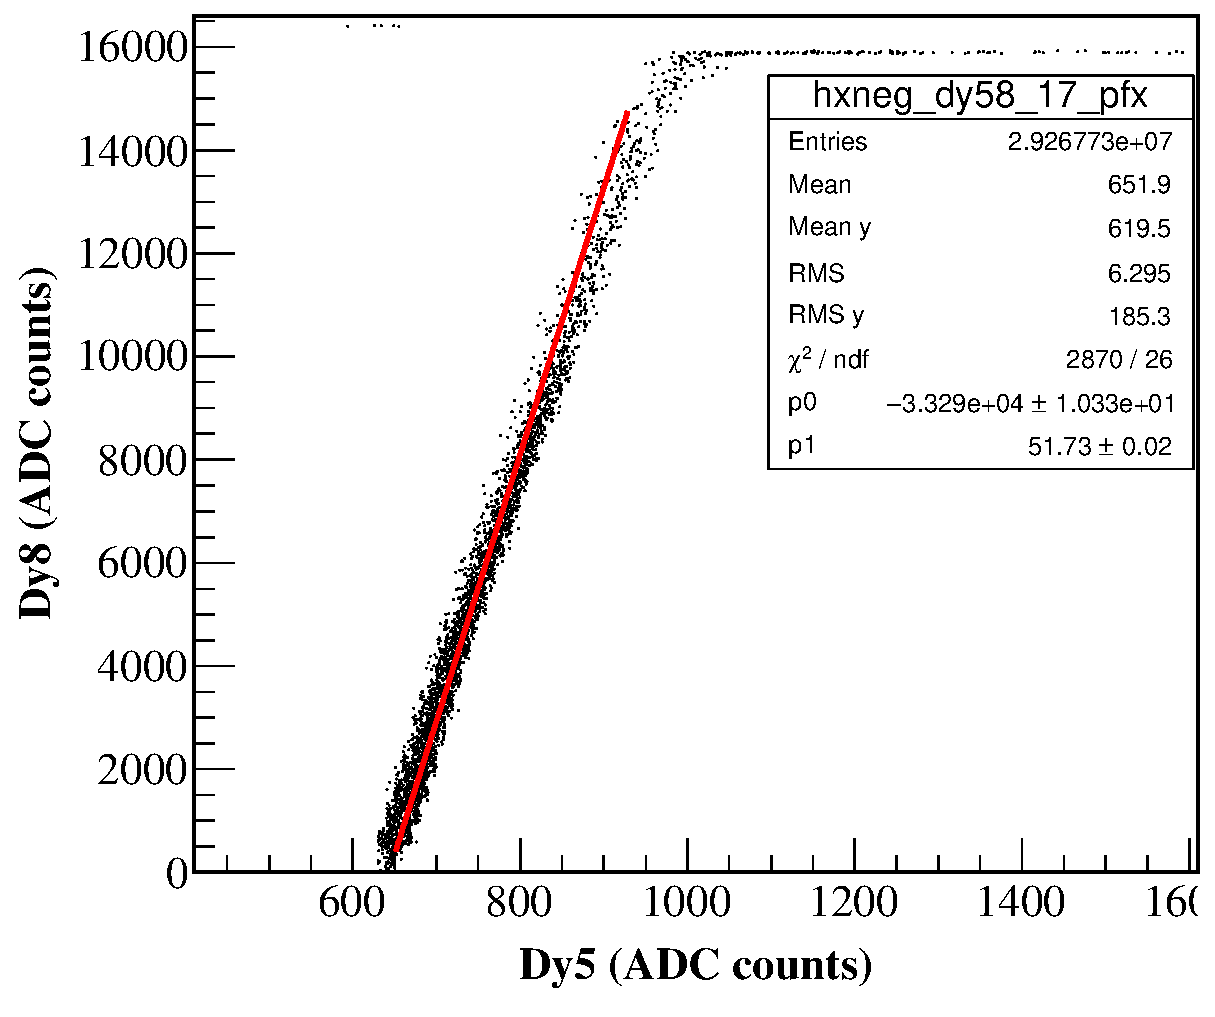
\includegraphics[width=0.48\textwidth]{chap/cosmic_ray/fig/dy58_example.eps}
}
\subfloat[][Dy58比值分布]{
	\label{fig:cosmic_ray:dy58_dist}
	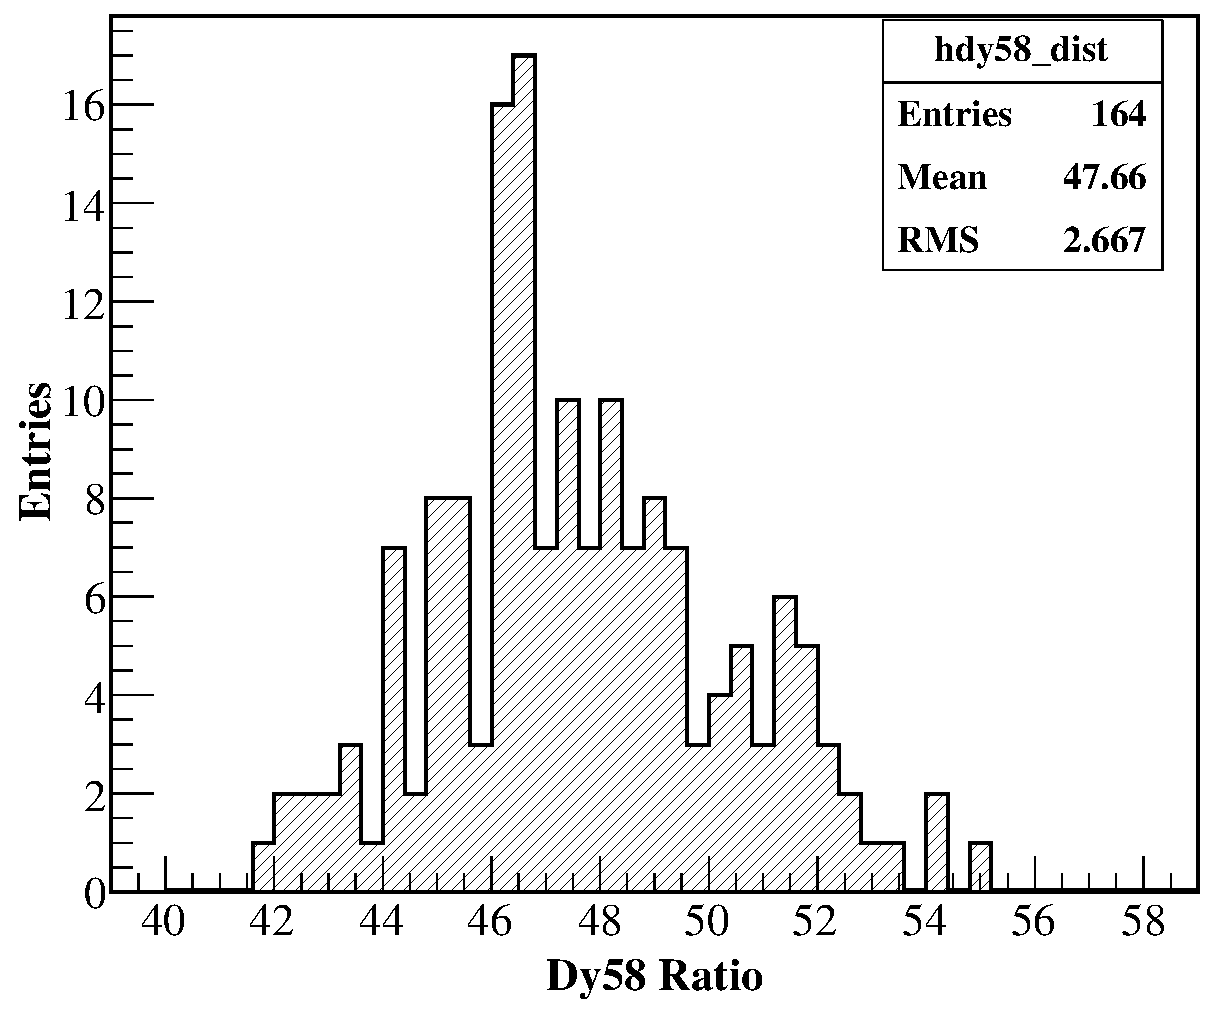
\includegraphics[width=0.48\textwidth]{chap/cosmic_ray/fig/dy58_dist.eps}
}
\caption{PSD宇宙线标定测试得到的Dy58比值结果}
\label{fig:cosmic_ray:dy58_results}
\end{figure}

使用相同的方法,我们得到了PSD所有探测单元模块正负两端的Dy58比值,结果如图\ref{fig:cosmic_ray:dy58_dist}所示。可以看到,Dy58比值分布较为集中,而均值在47左右。

\subsection{探测效率}
\label{sec:cosmic_ray:efficiency}
% 探测效率判据
% 事例筛选
% 结果分布
PSD探测单元模块的探测效率按照如下步骤分析得到:
\begin{enumerate}
	\item 对于每个有效事例,我么根据重建的入射宇宙线径迹,推出PSD上被击中的探测单元模块,并将该单元模块的击中事例数加1.
	\item 如果该单元模块被击中,我们以5倍的基线噪声($5\sigma$)为基准,判断该模块是否探测到该事例。如果该单元模块两端测得的信号幅度都大于$5\sigma$,则我们认为该事件被探测到,并将该探测单元模块的探测事例数加1;如果至少有一端的信号幅度小于$5\sigma$,我们则认为该事件没有被探测到,继续进行下个事例的处理。
	\item 上两个步骤循环反复,直到所有事例被处理完。
	\item 最后,我们将各个探测单元模块的探测事例数除以击中事例数,就得到了对应单元模块的探测效率。
\end{enumerate}
结果显示,PSD所有探测单元模块的探测效率都大于\SI{95}{\percent},因此满足PSD的设计要求,如图\ref{fig:cosmic_ray:efficiency}所示。
\begin{figure}[htbp]
	\centering
	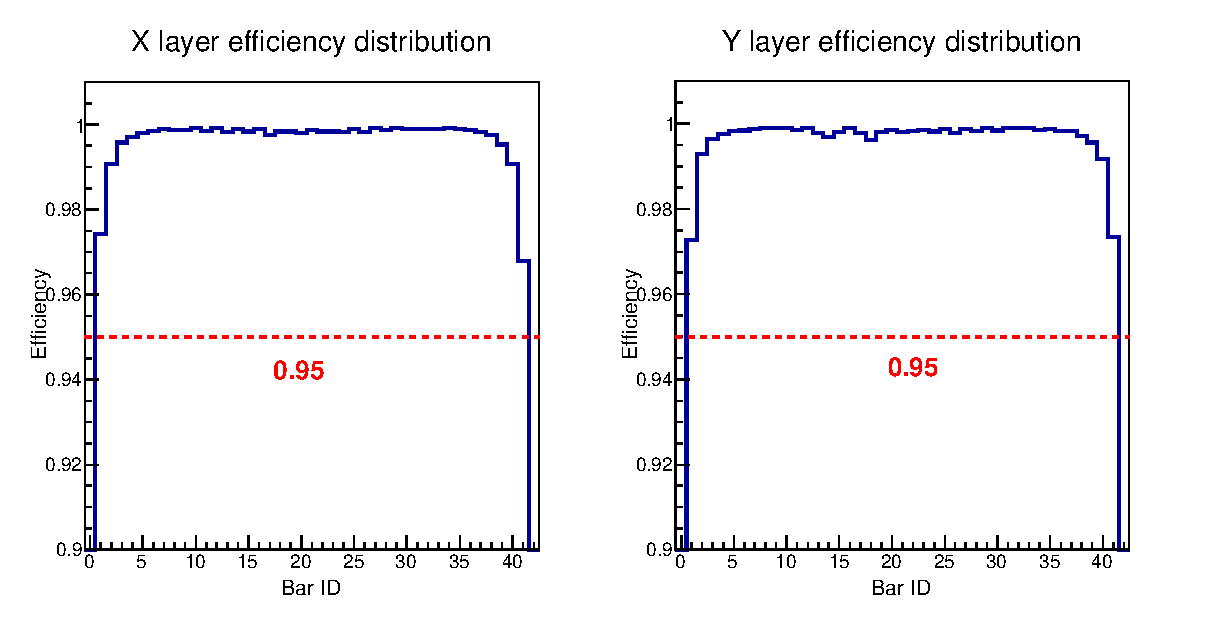
\includegraphics[width=0.95\textwidth]{chap/cosmic_ray/fig/efficiency.eps}
	\caption{PSD各探测单元模块的探测效率,左边是X层的结果,右边是Y层的结果}
	\label{fig:cosmic_ray:efficiency}
\end{figure}
可以看到,每一层中间位置的探测效率值远高于边缘位置的,这是由于边缘位置的击中事例数较少导致的。

\subsection{位置分辨}
\label{sec:cosmic_ray:position_resolution}
% 位置重建原理
% 结果
PSD的初步重建较为简单:1)依据\ref{sec:cosmic_ray:efficiency}节的判据,根据PSD自身的信息判断X层和Y层是否有单元模块被击中;2)若干X层和Y层都有单元模块探测到信号,就以它们交叠区域的中心位置作为PSD的宇宙线的击中位置坐标。
一般来讲,入射宇宙线能够分别在X层和Y层击中一个探测单元模块。
但由于每一层内相邻塑闪单元条之间有重叠区域,特殊情况下,入射宇宙线也会击中同一层内两根相邻的塑闪单元条,此时这两个探测单元模块都应该有击中信号。
在这种情况下,我们以相邻单元条的重叠区域中心值为重建位置坐标,从而能够提高位置测量的精度。

由于MWDC的位置测量精度远高于PSD的,我们可以认为根据MWDC重建的宇宙线入射径迹推出的PSD击中位置是真实的击中位置。
将上述PSD的重建位置坐标与该真实击中位置坐标相减,并将所有事例的结果累积起来,我们就能得到PSD的位置分辨率,结果如图\ref{fig:cosmic_ray:pos_resolution}所示。
可以看到,X层的位置分辨率为\SI{5.4}{mm},而Y层的位置分辨率为\SI{6.2}{mm},它们都满足PSD的设计要求。
\begin{figure}[htbp]
	\centering
	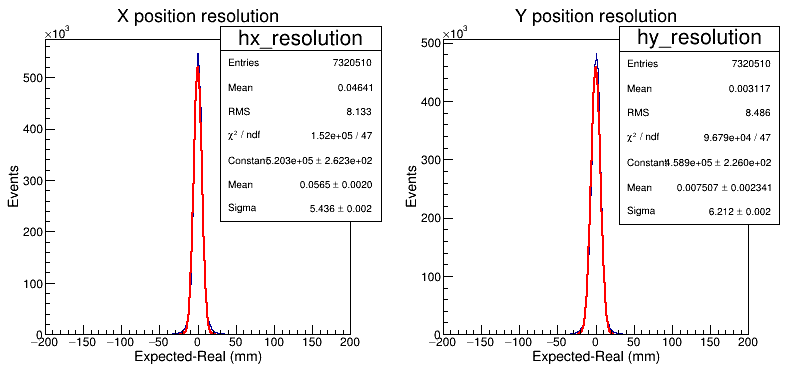
\includegraphics[width=0.95\textwidth]{chap/cosmic_ray/fig/pos_resolution.png}
	\caption{PSD两个探测平面的位置分辨}
	\label{fig:cosmic_ray:pos_resolution}
\end{figure}
% \section{PSD的物理量重建研究}
% \subsection{能量重建}
% \subsection{位置重建}